\subsection{Early Decisions for a Planned Encoder Update}\label{app:early_update}

On CIFAR-10~\citep{krizhevsky2009cifar}, we freeze the ResNet-18 prefix
and continue the final block for eight epochs. The deployed consumer is
the initial ten-class reader and its two confidence gates. We fit readers
with labels on $20\%$ of the $4{,}096$ fitting examples. The repair and
warning use $1{,}024$ unlabeled anchors and a separate $512$-example
monitor. Six confirmation references each have a separate
$2{,}000$-image evaluation partition.

The early monitor estimates the largest disagreement across the three
consumer rules. We compare forecasts obtained by scaling the change from
healthy features to epoch-two features. Across two development references,
the selected multiplier is one. Each confirmation run saves its risk
estimates and chosen repair family at epoch two, then resumes the same
optimizer and data-order state. At epoch eight, we fit the chosen family
on the original anchors and evaluate it alongside the unchanged head.

Among the $18$ planned updates, the unchanged head exceeds the $5\%$
budget in $17$. The epoch-two prediction has MAE $1.99$ points, compared
with $1.08$ for a predictor that uses only the learning rate and the
development mean for that schedule. With one safe update and the
persistence multiplier, the original forecasting gate fails. The original
early repair choices keep every held-out disagreement within budget,
using the full reference suffix for $12/18$ updates. Five of the $17$
unsafe cases use a repair with no reference suffix, below the prespecified
half-coverage target.

Before inspecting confirmation outcomes, we fix a separate stability
control and a limited-reference replay. The six lower-rate stability
runs all stay below budget. Across the $24$ updates, the early warning
detects $15/17$ exceedances and clears $7/7$ safe cases. Both misses are
mild updates, whose risk rises from $4.30\%$ to $6.85\%$ and from $4.49\%$
to $7.90\%$. These updates use moment repair in the limited-reference
replay.

The replay selects direct, moment, or ridge repair on the sealed
epoch-two monitor. It can also reserve exact reference calls for a fixed
fraction of low-margin examples. The policy uses a $2.5\%$ monitor
target and a $5\%$ held-out budget. It meets the latter on all $24$
updates, with a maximum of $4.10\%$. Its median reference fraction on
unsafe updates is $25\%$, compared with $75\%$ for uniform referral
under the same rule. At matched query fractions, margin ranking reduces
disagreement by $0.93$ points $[0.72,1.13]$. On the original $18$ updates,
mean reference use falls from $66.7\%$ to $38.3\%$.

Both old-output programs use the same current predictions. Completing
the update improves current accuracy by $1.45$ points $[1.06,1.84]$
over stopping at epoch two. At the nominal learning rate, joint
continuation and the matched supervised control have the same mean
accuracy, with difference $0.00$ points $[-0.12,0.12]$. The auxiliary
loss ratio is $0.980$ $[0.977,0.982]$. Intervals use the six reference
means. Reference calls measure access in the batched replay.

\begin{figure}[H]
\centering
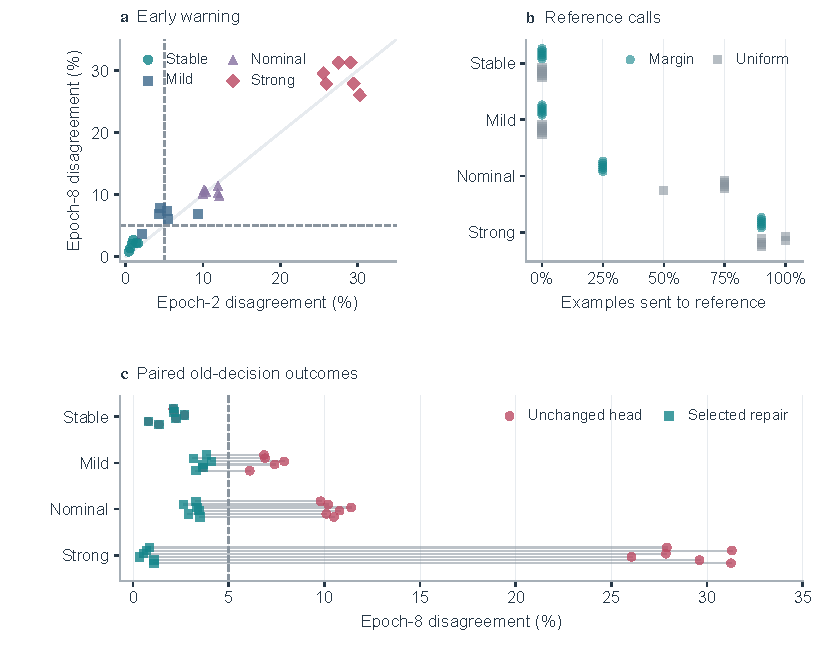
\includegraphics[width=\linewidth]{figures/fig_early_update.pdf}
\caption{Early decisions on CIFAR-10 with ResNet-18. Each point is one
planned update of a fitted reference. (a) Maximum direct disagreement at
epochs two and eight. The dashed lines mark the $5\%$ limit.
(b) Reference fractions fixed by the epoch-two replay for margin and
uniform referral. (c) Paired held-out disagreement for the unchanged
head and the selected margin policy.}
\label{fig:early_update}
\end{figure}
